% !TeX root = ../thuthesis-example.tex

\chapter{引言}


\section{研究背景}\label{1-background}

\subsection{工业物联网和时序数据}
物联网(Internet of Things, IoT)的概念最初于1999年提出,通常指使用网络连接多种信息感知设备,实现信息交换,从而让系统能够自动地、实时地对物体进行识别、定位、追踪、监控并触发相应事件\cite{王保云2009物联网技术研究综述木}。目前,应用物联网的领域包括智能家居、可穿戴设备、工业物联网、智慧医疗、智慧城市、智慧农业等。根据相关研究,2025年全球GDP的4\% - 11\%将由物联网贡献\cite{mouha2021internet}。

工业物联网(Industrial Internet of Things, IIoT)\cite{sisinni2018industrial}是物联网的一个细分领域,通过在工业领域部署传感器、仪器、设备和其他物联网装置,依赖数据采集、传输、分析处理和应用等完成工业流程、实现效率提升,完成新型商业模式的构建,推动传统工业向数字化、智能化的转型升级,在智能制造、能源领域、物流运输、医疗保健、农业领域等都有着广泛的应用。

在工业物联网中,时间序列数据(Time-Series Data)\cite{dunning2015tsdb}扮演着至关重要的角色。在时序数据中,每个数据点都与一个特定的时间戳相关联,表明该数据是在何时被记录或观测到的。工业环境中部署的各种传感器、仪器和设备会持续不断地产生大量的时序数据。时序数据具备以下特点:

1. 产生速度快。工业设备上的各种传感器,如温度传感器、振动传感器、压力传感器等,能在每秒甚至每毫秒产生多个数据点。一条生产线上可部署成百上千个传感器,瞬间产生大量数据。举例来说,国际风电标准 IEC 61400-25 规定,一台风机每秒需要采集 225KB 的工业数据,在某些极端工况下数据的采集频率需要提升至 8 KHz\cite{PZKX202005001},即每秒产生八千次的采样。

2. 总量巨大。时序数据以较高的频率持续产生,并且往往需要长期保存以进行历史分析、趋势预测等,因此其累积的总量往往非常庞大。举例来说,长安汽车集团的车联网会为每一辆生产的汽车部署数千个传感器,每年产生的原始数据量超过13PB。

3. 种类丰富。按照应用的领域划分,不同行业关注不同的时序数据指标。例如,工业领域关注设备运行参数,金融领域关注交易价格和成交量,医疗领域关注生理指标,环境监测领域关注污染物浓度等。按照数据的特点划分,时序数据可以分为数值型数据(例如温度、压力、速度)、布尔型数据(例如设备的开/关状态)、离散型数据(例如故障代码)甚至文本型数据(例如日志信息)等。


\subsection{时序数据库和Apache IoTDB}

时序数据库\cite{naqvi2017timeseriesdb}是针对管理时序数据而优化的数据管理系统。相较于关系性数据库\cite{codd2007relational}和NoSQL数据库\cite{han2011surveynosql},时序数据库通常具备更低的写入延迟、更高的写入吞吐、更强的存储压缩能力、更高效的时间范围查询和聚合能力等。在实现上,时序数据库通常采用LSM\cite{o1996lsmtree}引擎进行数据存储,内置丰富的基于时间窗口的聚合查询函数、专门的压缩算法等。
常见的时序数据库包含Apache IoTDB\cite{wang2020iotdb}、InfluxDB\cite{shahid2019influxdb}、TDEngine\cite{tdengine_website}、DolphinDB\cite{dolphindb_website}、OpenTSDB\cite{opentsdb_website}、TimescaleDB\cite{timescale_website}等。

Apache IoTDB是一个开源的分布式时序数据库,目前是Apache基金会的顶级项目,具有为时间序列数据优化的存储引擎、查询引擎以及分布式框架。Apache IoTDB能够满足海量工业物联网时序数据的高吞吐低延时写入、高压缩比存储、快速查询和复杂分析的需求,凭借着高性能、高可用性等特点在工业物联网、智能城市、智能电网等领域得到广泛应用。

Apache IoTDB 集群节点包括数据节点(DataNode)和管理节点(ConfigNode)。数据节点
负责管理数据分区(DataRegion)和元数据分区(SchemaRegion),管理节点负责管理集群节点、信息分区(PartitionRegion)、负载均衡、分布式调度等。客户端可以通过会话(Session)连接到集群的数据节点执行请求。

在Apache IoTDB这样的分布式数据库中,高可用和容错能力\cite{gray2002high}是确保用户业务连续性的至关重要的指标。数据库系统的故障和服务的中断可能会导致数据丢失、经济损失、企业声誉受损,甚至会引发严重的安全风险。
恢复时间目标(Recovery Time Objective, RTO) 和恢复点目标 (Recovery Point Objective, RPO) \cite{suguna2014overview}是衡量高可用性的两个重要指标。RTO 是指从服务中断到恢复服务所需的最长可接受时间,而 RPO 是指在发生中断后可能丢失数据的最大可接受时间。Apache IoTDB在高可用和容错能力的建设目标就是追求RPO为零、RTO尽可能短。

目前Apache IoTDB围绕高可用性和容错能力已经实现包括:

1. 建立统一的共识协议框架,为数据维护多个副本,避免因单点故障导致的数据永久性丢失的问题。
通过统一的接口建设,IoTDB还实现了性能和一致性级别不同的各类共识协议,包括基于强一致性协议的RatisConsensus、基于会话一致性的IoTConsensus和基于最终一致性的IoTConsensusV2。
从RatisConsensus到IoTConsensus到IoTConsensusV2,IoTDB在牺牲一致性的基础上,获得显著的性能提升,更加符合工业物联网时序场景的需要。

2. 建立故障检测机制。IoTDB的管理节点领导者会定期跟所有其他节点(管理节点、数据节点)交换心跳,心跳的内容包括节点的存活与否、负载情况、磁盘用量等。
通过心跳的内容和心跳超时的机制,管理节点领导者可以判断节点失效和磁盘写满的故障。当管理节点领导者发现某个数据节点长时间不响应心跳,会判断这个节点失效,发出警告,并影响后续的分区决策、负载均衡决策、客户端的连接决策等。当管理节点领导者发现某个节点磁盘告警,则会将该节点以及节点上所有的数据副本设置成为只读状态,只能服务查询请求,拒绝所有的写入请求。

3. 建立故障恢复和故障切换的机制。IoTDB的客户端能够在数据节点失效时将请求重新引导到其他存活的数据节点进行重试。在查询和写入执行时,IoTDB的协调者(Coordinator)能够挑选那些存活的副本进行请求的执行,避开故障的副本。同时,对于失败的查询请求还会允许用户配置重试策略,来规避瞬时的故障。


\subsection{研究问题}\label{1-motivation}

当前 Apache IoTDB 在应对非对称网络分区等复杂分布式故障模式时,其自动故障检测、故障恢复及\failover 机制仍有进一步完善的空间:

1. 故障检测不完全,无法检测非对称网络分区等故障。在系统出现非对称网络分区故障时,系统无法意识到故障,出现性能退化,无法自动恢复。在两副本RatisConsensus中,若主副本和从副本分属非对称网络分区的两个节点,那么从副本会主动发起无限期选举操作,无法接受任何请求。在查询和写入调度的时候,依然有可能会将请求转发到非对称分区的从副本上进行重试,导致系统整体的吞吐下降。

2. 故障从发生到被发现的检测时间较长、机制单一僵硬。IoTDB目前通过固定的心跳超时(默认为20s)对节点存活情况进行判断。固定的20秒超时无法适应不同应用场景、动态变化的网络状况和系统负载,在系统网络不稳定、负载较高的情况下会产生误判,导致不必要的\failover 和系统资源浪费。

3. 自动错误转移和恢复机制不完善。目前,写入请求无法在副本失效时自动转移到其他副本上执行操作。在部分由于故障集群导致组件失效场景下,即使系统的存活组件依然能够为查询请求提供服务,但在制定查询和写入策略时无法充分利用这些健康的资源,无法自适应进行自动错误的转移,影响系统的整体性能和可用性。

因此,本文的核心研究问题在于:总结分布式系统故障的共性,提出并实现Apache IoTDB高可用性和容错能力的通用框架,确保系统能够在进程宕机、网络分区等场景下迅速检测错误、从错误中切换和恢复,保证系统能够持续、可靠地提供时序数据服务。

本文的研究具备以下意义:

1. 确保用户工业应用的业务连续性。高可用的 IoTDB 系统能够最大限度地减少因系统故障导致的停机时间,确保工业设备数据的持续采集、存储与查询,从而有力支撑实时监控、预测性维护、运营优化等关键工业应用,满足客户对数据服务的高标准需求,防止用户因为业务中断而产生经济损失、安全风险和声誉受损。

2. 保证用户的数据安全。高可用和容错通过为用户数据备份,消除单点故障,保证用户的数据资产的安全性和可靠存储。

3. 提升系统可信赖度与推广价值:在对数据可靠性与系统稳定性要求极高的工业领域,高可用性和可用能力能够帮助Apache IoTDB通过相关的评估测试,增强其在工业、能源、交通等关键行业应用中的竞争力与吸引力,推动其更广泛的落地和应用。



\section{研究内容}


本文的研究工作旨在为Apache IoTDB构建完善且极致的高可用能力,来应对日益复杂的工业物联网应用场景。

高可用能力的构建原则是,无论发生的故障类型是什么,都能够被正确诊断,且只要集群中仍然存活的组件能够完成用户请求,那么就该通过\failover 和容错的设计继续服务这些请求。

高可用能力的构建目标是,实现 RPO 为零,即在故障发生时,不会丢失任何已提交的数据;并达到RTO为分钟级,意味着系统能够在极短的时间内完成故障的转移和恢复,最大限度地减少服务中断对业务的影响。

高可用能力的构建方式是,实现对集群故障的更早、更全面、更准确地检测与研判,并通过集群现有能力的深度协同与优化,更快、更鲁棒的方式进行故障的转移和自动恢复,提升系统的整体韧性和弹性。

为实现高可用能力,本文的主要工作包括:

1. 对Apache IoTDB面临的故障场景整体研究。
本文将深入分析分布式系统中可能出现的各种故障类型,包括但不限于节点失效、网络异常、存储故障、软件缺陷以及人为错误等,并识别这些故障的共性特征和潜在影响。在此基础上,本文将通过提出完整的高可用性方法论和架构,定义系统的高可用关键组件、交互方式以及应对不同故障场景的策略,形成一套基于故障检测、故障恢复和\failover 的高可用性框架。

2. 实现高可用性框架的算法。Apache IoTDB高可用性和容错能力基于故障检测、故障转移和故障恢复。通过集群节点相互的状态感知、基于状态感知的故障研判算法实现故障的及时发现;通过共识协议的多副本能力和读写请求规划、执行和重试实现\failover;通过共识协议的数据同步实现故障副本的重启恢复。最终在整体上提升IoTDB分布式系统的韧性,使其能够应对更广泛的故障场景。建设目标如图\ref{fig:c01-overview-arch}所示。


\begin{figure}
  \centering
  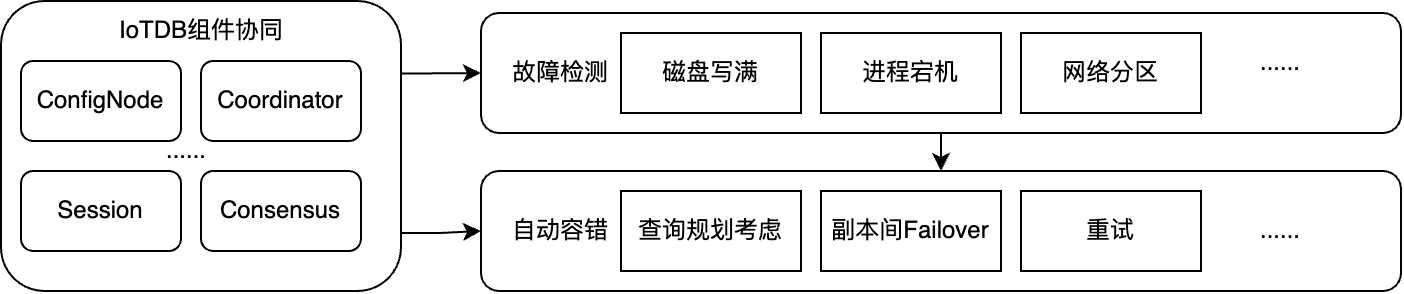
\includegraphics[width=0.99\linewidth]{1-overview-arch.png}
  \caption{IoTDB整体的高可用框架设计}
  \label{fig:c01-overview-arch}
\end{figure}

3. 对提出的高可用框架设计和实现进行测试和验证。本文将设计一系列覆盖各种故障场景的测试用例,包括模拟节点失效、网络分区、磁盘故障等。测试将关注系统的故障检测速度、恢复时间、数据一致性以及对系统整体性能的影响等方面。通过严谨的实验和数据分析,我们将验证所构建的高可用性架构是否能够达到预期的目标。



\section{主要贡献}

本文的贡献主要体现在以下几个方面:

1. 对分布式时序数据库在运行中潜在的故障进行系统性的梳理、分类和分析。本文将种类繁多的故障总结为节点宕机、磁盘资源不足、网络分区(对称分区和非对称分区)、集群状态短暂不一致五类,并分析每一种故障的原因、对系统的影响。这项工作是后续设计高可用和容错框架的问题基础。

2. 提出针对 Apache IoTDB 系统的高可用与容错框架。该框架依赖共识协议提供的基础能力,划分为故障检测、故障恢复、\failover 三部分。框架明确系统各组件,即客户端、管理节点、数据节点之间的协同机制。

3. 上述工作在Apache IoTDB系统中进行实现,并在测试环境中对框架能力做全面测试与评估。针对1中提出的五类故障场景,系统实现的故障容错机制能够有效工作,并实现RPO指标为零、RTO指标为分钟级的目标。


\section{组织结构}
本文共分为8个章节,每个章节的内容如下:

第1章为引言部分,介绍了工业物联网、时间序列数据、时序数据库、Apache IoTDB、分布式数据库中的高可用性和容错能力等背景,阐述本文建设更极致、更完善的可用性的研究动机,概括本文的研究内容和研究贡献,描述本文的组织结构。

第2章为相关工作,重点介绍学术界对于分布式系统故障、高可用容错相关的研究,Apache IoTDB现有的共识模块的能力,以及工业界多个广泛应用的分布式系统如Apache Cassandra、TiDB和OceanBase中的高可用方案的介绍。

第3章介绍了常见的分布式故障的特性和共性,包含进程宕机、磁盘写满、网络分区和集群变更的短暂不一致性。基于这些故障,第三章提出Apache IoTDB的高可用和容错框架,包含故障检测、\failover 和故障转移。

第4章介绍了集群的故障检测和发现机制,包括管理节点、数据节点和客户端之间对其他系统组件基于心跳的状态感知能力,以及基于心跳历史的的故障研判算法,包括固定心跳超时、Phi Accrual算法、基于Thrift连接状态的算法。

第5章介绍了集群的故障恢复和容错能力,基于客户端、管理节点和数据节点的组件协同,覆盖请求规划、请求执行和请求重试三个阶段,实现对故障的转移和恢复。

第6章介绍了集群对于经典故障场景的容错流程。结合第4章的故障检测和发现机制、第5章的故障恢复和容错机制,IoTDB集群能够抵御第3章列举的磁盘写满、进程宕机、网络对称/非对称分区、集群变更时的不一致等问题,并给出每种场景的详细容错流程。

第7章为实验部分。实验验证了优化后的故障检测能力,给出不同的共识协议在高可用能力方面的比较,并且针对第6章的故障场景验证集群的RPO和RTO指标、故障时期的吞吐情况。

第8章总结本文的工作和不足之处,并指出未来工作的主要方向。